\documentclass[a1]{sciposter}
\usepackage{epsfig}
\usepackage{amsmath}
\usepackage{amssymb}
\usepackage{multicol}
\usepackage{graphicx,url}
\usepackage[portuges, brazil]{babel}   
\usepackage[utf8]{inputenc}
\usepackage[sfdefault]{FiraSans} 
\usepackage{inconsolata}
\usepackage[T1]{fontenc}
\renewcommand*\oldstylenums[1]{{\firaoldstyle #1}}
\usepackage[cm]{sfmath}
\usepackage{tcolorbox}
\usepackage{xcolor}
%\usepackage{fancybullets}
\usepackage{subfig}
\usepackage{graphicx}
\newtheorem{Def}{Definition}

\newcommand\kcont{\protect\mathpalette{\protect\independenT}{\perp}}
\def\independenT#1#2{\mathrel{\rlap{$#1#2$}\mkern2mu{#1#2}}}

\newcommand{\krev}{\downarrow\downarrow}

% create subfigure environment
\def\subfigure{\let\oldcaption=\caption
\let\caption=\subcaption
\minipage}
\def\endsubfigure{\endminipage
\let\caption=\oldcaption}

\newcommand{\subcaption}[1]% %1 = text
{\refstepcounter{subfig}%
\par\vskip\abovecaptionskip
\centerline{\textbf{(\alph{subfig})} #1}%
\vskip\belowcaptionskip\par}

\urlstyle{same}

\title{Filtragem de Ruído Telúrico em Sinais Astronômicos}
%Título do projeto

\author{
Isabela Blücher \\
Orientadora: Prof.ª Dra. Paula Rodrigues Teixeira Coelho\\
Coorientador: Prof. Dr. Marcelo Gomes de Queiroz\\}
%nome dos autores

\institute 
{Instituto de Matemática e Estatística \\
 Universidade de São Paulo}
%Nome e endereço da Instituição

% \email{isabela.blucher@usp.br}
% Onde você coloca os emails dos integrantes

\rightlogo[1.2]{usp-logo-png}
\leftlogo[1]{ime}
% Exibe os logos (direita e esquerda) 
% Procure usar arquivos png ou jpg, e de preferencia mantenha na mesma pasta do .tex
%%%%%%%%%%%%%%%%%%%%%%%%%%%%%%%%%%%%%%%%%%%%%%%%%%%%%%%%%%%%%%%%%%%%%%%%%%%%%%%%
%%% Begin of Document

\begin{document}
%define conference poster is presented at (appears as footer)

%\LEFTSIDEfootlogo  
% Uncomment to put footer logo on left side, and 
% conference name on right side of footer

% Some examples of caption control (remove % to check result)

%\renewcommand{\algorithmname}{Algoritme} % for Dutch

%\renewcommand{\mastercapstartstyle}[1]{\textit{\textbf{#1}}}
%\renewcommand{\algcapstartstyle}[1]{\textsc{\textbf{#1}}}
%\renewcommand{\algcapbodystyle}{\bfseries}
%\renewcommand{\thealgorithm}{\Roman{algorithm}}

\maketitle

%%% Begin of Multicols-Enviroment
\begin{multicols}{2}

%%% Abstract
\section{Introdução}

Estrelas são corpos celestes que emitem energia na forma de radiação eletromagnética. Esta energia alcança a superfície terrestre e interage com moléculas presentes na atmosfera, como oxigênio e vapor de água.\\

O sinal estelar é capturado a partir do solo por instrumentos denominados espectrógrafos, que dividem a radiação eletromagnética emitida pela estrela em seus comprimentos de onda. Esta captura resulta em um espectro: um mapa de radiação em função do comprimento de onda.\\

A interação da atmosfera com a observação estelar resulta em um espectro distorcido e contaminado, devido à formação de novas linhas espectrais no espectro capturado instrumentalmente, denominadas linhas telúricas.\\

Neste trabalho foram estudados métodos existentes de correção telúrica e potenciais soluções computacionais que sejam capazes de remover ou atenuar a contaminação telúrica de espectros estelares capturados a partir do solo.

\section{Contaminação Telúrica}

Em termos matemáticos, o problema da contaminação telúrica pode ser descrito como: consideramos os vetores $o$ (observado), $a$ (atmosfera) e $s$ (estrela), que representam os espectros observado, telúrico e estelar sem contaminação. Podemos representar a contaminação telúrica pela equação
\begin{equation*}
    o = a \circ s \qquad \left(\mbox{ou equivalentemente:} \qquad o_i = a_i\cdot s_i,\ \forall i\right).
\end{equation*}

Devido a natureza multiplicativa do problema, a correção telúrica dos espectros observados seria a divisão simples do espectro observado pelo telúrico. Porém, esta formulação do problema pressupõe que as três sequências estão perfeitamente alinhadas, o que não corresponde à realidade.

\section{Correção Telúrica}

Foi feito um experimento para testar o método da correção telúrica pela divisão simples dos espectros, de modo a observar que na prática esta solução não é ideal e cria artefatos no espectro estelar observado.

\begin{figure}
 \centering
 \begin{subfigure}{0.4\textwidth}
  \centering
  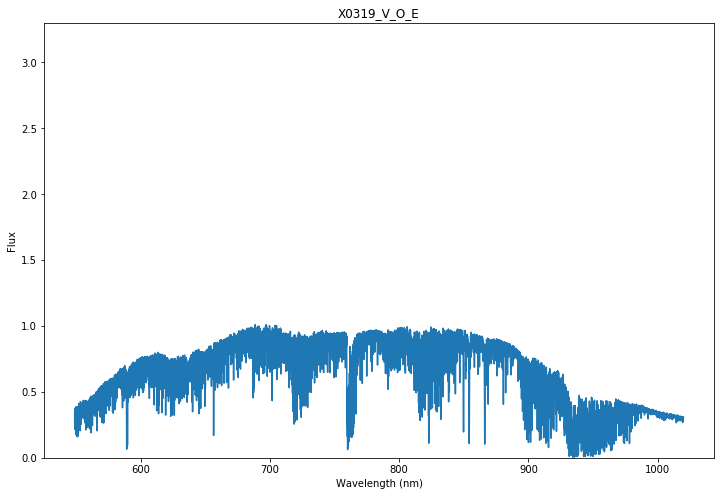
\includegraphics[width=1.1\textwidth]{x0319_v_o_e_scaled.png}
  \caption{X0319}
 \end{subfigure}\hfil
 \begin{subfigure}{0.4\textwidth}
  \centering
  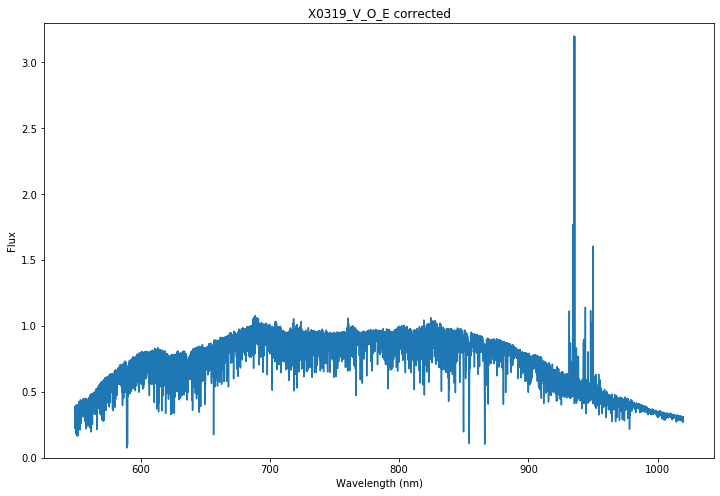
\includegraphics[width=1.1\textwidth]{x0319_v_o_e_divided.png}
  \caption{Correção telúrica de X0319}
 \end{subfigure}\hfil
%   \caption{fig}
\end{figure}

A divisão da estrela X0319 por seu referencial telúrico correspondente ilustra as dificuldades deste método de correção telúrica, são observados picos no sinal que não deveriam existir na situação ideal do problema.

\section{Aplicação do \textit{Dynamic Time Warping}}



\section{Conclusões}


\end{multicols}

\end{document}